% TLDR: ICML 2026 Math-AI workshop poster (61x91 cm portrait, Stanford gemini theme, XeLaTeX) for
% "CertJudge: Evaluating Lean Formal-Code With Falsifiable Properties".
% Compile: latexmk -xelatex -interaction=nonstopmode main.tex
% Design per ~/agents-config/writing/ml_research/write-poster.md (Rylan Schaeffer rules):
% motivation / clear intuitive results / takeaway; <=800 words; figures carry the content.

\documentclass[final]{beamer}

% ====================
% Packages
% ====================

\usepackage[T1]{fontenc}
\usepackage{lmodern}
\usepackage[size=custom,width=61,height=91,scale=1.0]{beamerposter}
\usetheme{gemini}
\usecolortheme{stanford}
% Highlighted (alert) blocks: cardinal title bar + faint red body so the two key
% blocks pop for the walk-by reader (stanford color theme leaves these unset).
\setbeamercolor{block alerted title}{fg=white,bg=cardinalred}
\setbeamercolor{block alerted separator}{bg=cardinalred}
\setbeamercolor{block alerted body}{fg=black,bg=cardinalred!7}
\usepackage{amsmath}
\usepackage{graphicx}
\usepackage{booktabs}
\usepackage{tikz}
\usepackage{qrcode}

% ====================
% Lengths
% ====================
% (N+1)*\sepwidth + N*\colwidth = \paperwidth ; portrait 2-column: 3*0.03 + 2*0.455 = 1.0
\newlength{\sepwidth}
\newlength{\colwidth}
\setlength{\sepwidth}{0.03\paperwidth}
\setlength{\colwidth}{0.455\paperwidth}

\newcommand{\separatorcolumn}{\begin{column}{\sepwidth}\end{column}}
\newcommand{\tivar}{\ensuremath{\mathrm{TI}_{\mathrm{var}}}}

% ====================
% Title / authors
% ====================

\title{CertJudge: Evaluating Lean Formal-Code With Falsifiable Properties}

% TODO: CONFIRM AUTHOR LIST before printing — inferred from repo contributors, paper is anonymized
\author{Brando Miranda \inst{1,\dag} \and Ethan S.~Hersch \inst{1} \and Sanmi Koyejo \inst{1}}
\institute[Stanford]{\inst{1} Stanford University \qquad \inst{\dag} \texttt{brando9@stanford.edu}}

% ====================
% Footer
% ====================

\footercontent{
  \href{mailto:brando9@stanford.edu}{brando9@stanford.edu} \hfill
  ICML 2026 Math-AI Workshop \hfill
  \href{https://github.com/brando90/cert-judge}{github.com/brando90/cert-judge}
  \quad {\small\emph{[Author list to be confirmed]}}}

% ====================
% Logo (reserves headline space so the title stays clear of it)
% ====================

\logoright{
\includegraphics[height=5.5cm]{stanford_logos/Block_S_2_color.png}}

% ====================
% Body
% ====================

\begin{document}

\begin{frame}[t]
\begin{columns}[t]
\separatorcolumn

% ============================================================
% LEFT COLUMN — motivation, key idea, method
% ============================================================
\begin{column}{\colwidth}

  % CS197 moves 1-2: status quo (per-judge human validation) + why it fails at agent throughput
  \begin{block}{Validating LLM judges one human study at a time does not scale}

    \begin{itemize}
      \item AI agents now write Lean~4 code \textbf{and} the theorems/specs meant to verify it --- far faster than humans can inspect.
      \item The Lean kernel checks \emph{proofs}, not whether the \emph{right theorem} was proposed: a candidate can compile yet be under-specified, vacuous, or semantically shifted.
      \item So an LLM judge scores each candidate against a gold reference --- but every new judge, prompt, model, or threshold demands a \textbf{fresh human-agreement study}.
    \end{itemize}

    \smallskip
    {\centering\itshape Can one human calibration be amortized across future judges,\\ via checks that are automatic and falsifiable?\par}

  \end{block}

  % CS197 move 3: the flip — certify with falsifiable behavioral checks instead of re-labeling
  \begin{alertblock}{Key idea: certify the judge --- don't re-label it}

    \begin{itemize}
      \item \textbf{CertJudge}: humans rate a small panel \textbf{once} ($n{=}75$ candidate--gold Lean pairs); every new judge configuration is then screened by \textbf{automatic, falsifiable property checks}.
      \item Controlled perturbations test four behaviors, aggregated into a \textbf{variance-aware trust index} \tivar.
      \item Judges with higher \tivar{} agree more with humans --- certification predicts \emph{which judge to trust}, with no new labels.
    \end{itemize}

  \end{alertblock}

  % CS197 move 4: method/system — money figure carries it
  \begin{block}{Four falsifiable properties $\rightarrow$ one trust index}

    \begin{figure}
      \centering
      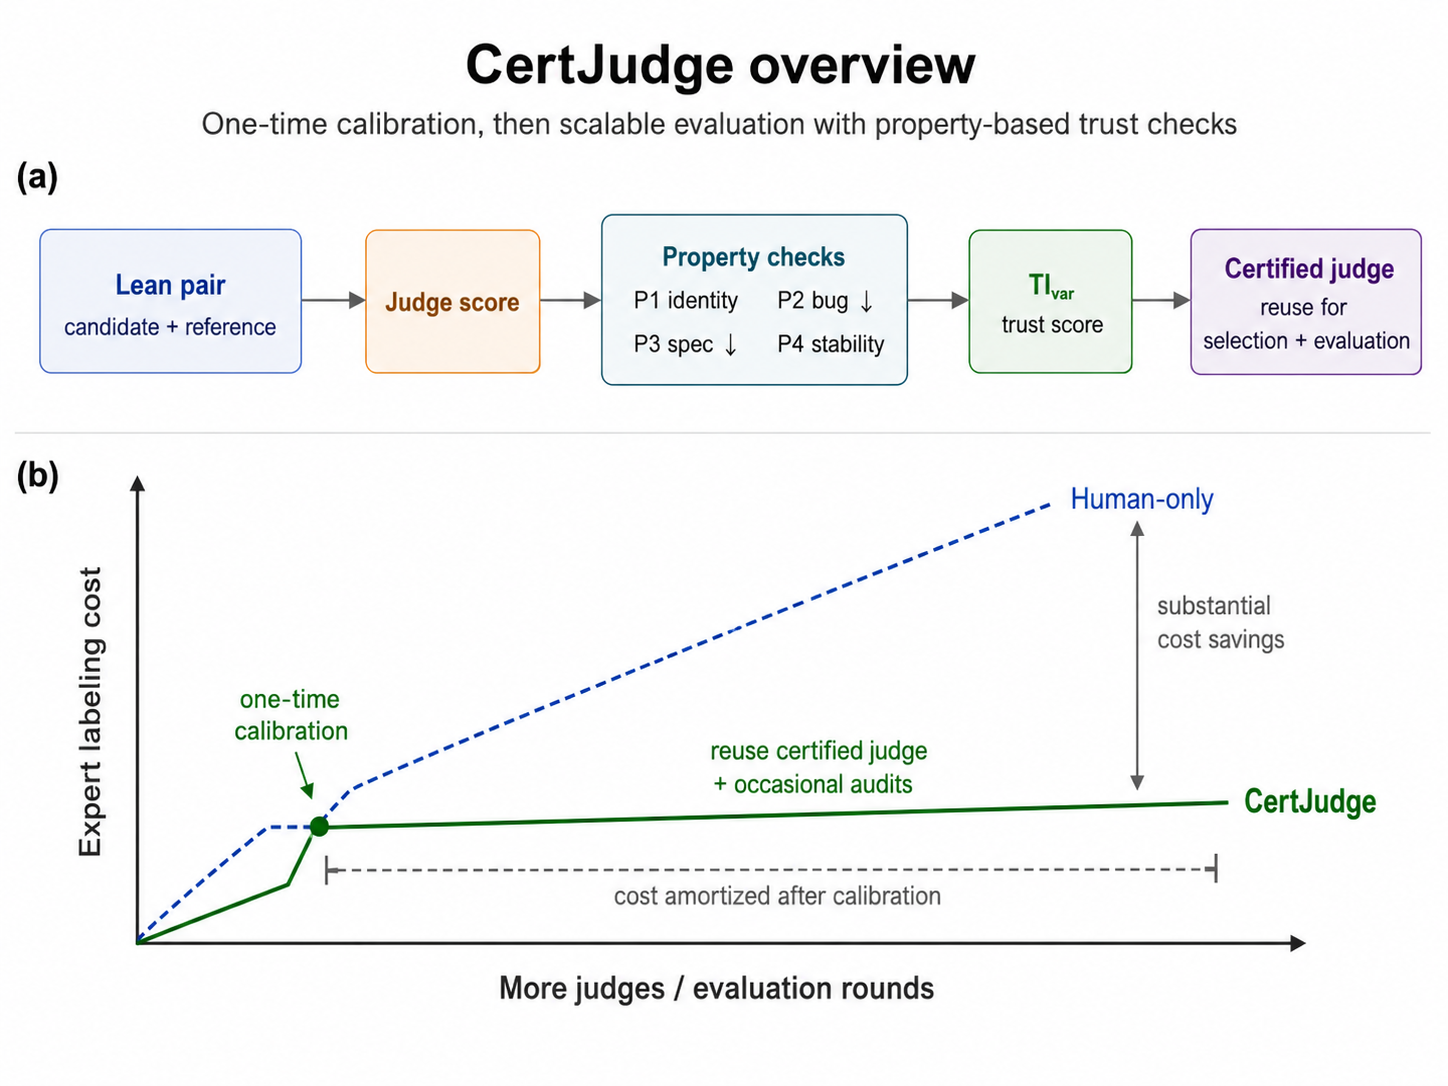
\includegraphics[width=0.86\linewidth]{figures/pull_fig.png}
      \caption{Label once, then certify automatically: property checks plus \tivar{} replace per-judge human studies, so labeling cost stops growing with the number of judges.}
    \end{figure}

    \begin{itemize}
      \item \textbf{P1 Identity:} $s(X,X)=1$ --- an artifact scored against itself gets the maximum.
      \item \textbf{P2 Bug monotonicity:} score falls as semantic bugs are injected.
      \item \textbf{P3 Spec monotonicity:} score falls as theorems/tests are removed.
      \item \textbf{P4 Stability:} score invariant across repeats and semantics-preserving rewrites.
    \end{itemize}

    \[
      \tivar = \exp\!\Big(
      \tfrac{1}{3}\log C_f
      + \tfrac{1}{3}\log(1-\widetilde{\mathrm{VarCorr}})
      + \tfrac{1}{3}\log(1-\widetilde{\mathrm{VarScore}})
      \Big)
    \]

    $C_f$: geometric aggregate of P1--P4; the variance terms penalize unstable judges. Multiplicative: \textbf{one failed property collapses the index}.

    \heading{Calibration setup}
    \textsc{VeriBench} Lean~4 artifacts \cite{anonymous2026veribench}: $n{=}75$ aligned candidate--gold pairs from 24 problems (3 agent generations per problem), two human passes each on a 0--5 rubric. 8 judge configurations per family: GPT-5.3-Codex, Claude Opus 4.7, Qwen3-Coder.

  \end{block}

\end{column}

\separatorcolumn

% ============================================================
% RIGHT COLUMN — results, takeaways, references
% ============================================================
\begin{column}{\colwidth}

  % CS197 move 5: headline result — big number + scatter
  \begin{block}{Result: \tivar{} predicts judge-level human alignment}

    {\centering
      {\Huge $\boldsymbol{\rho = 0.833}$}\\[1.2ex]
      validation-set Spearman between \tivar{} and human agreement\\
      (avg labels; $0.905$ pass1, $0.738$ pass2)\par
    }

    \begin{figure}
      \centering
      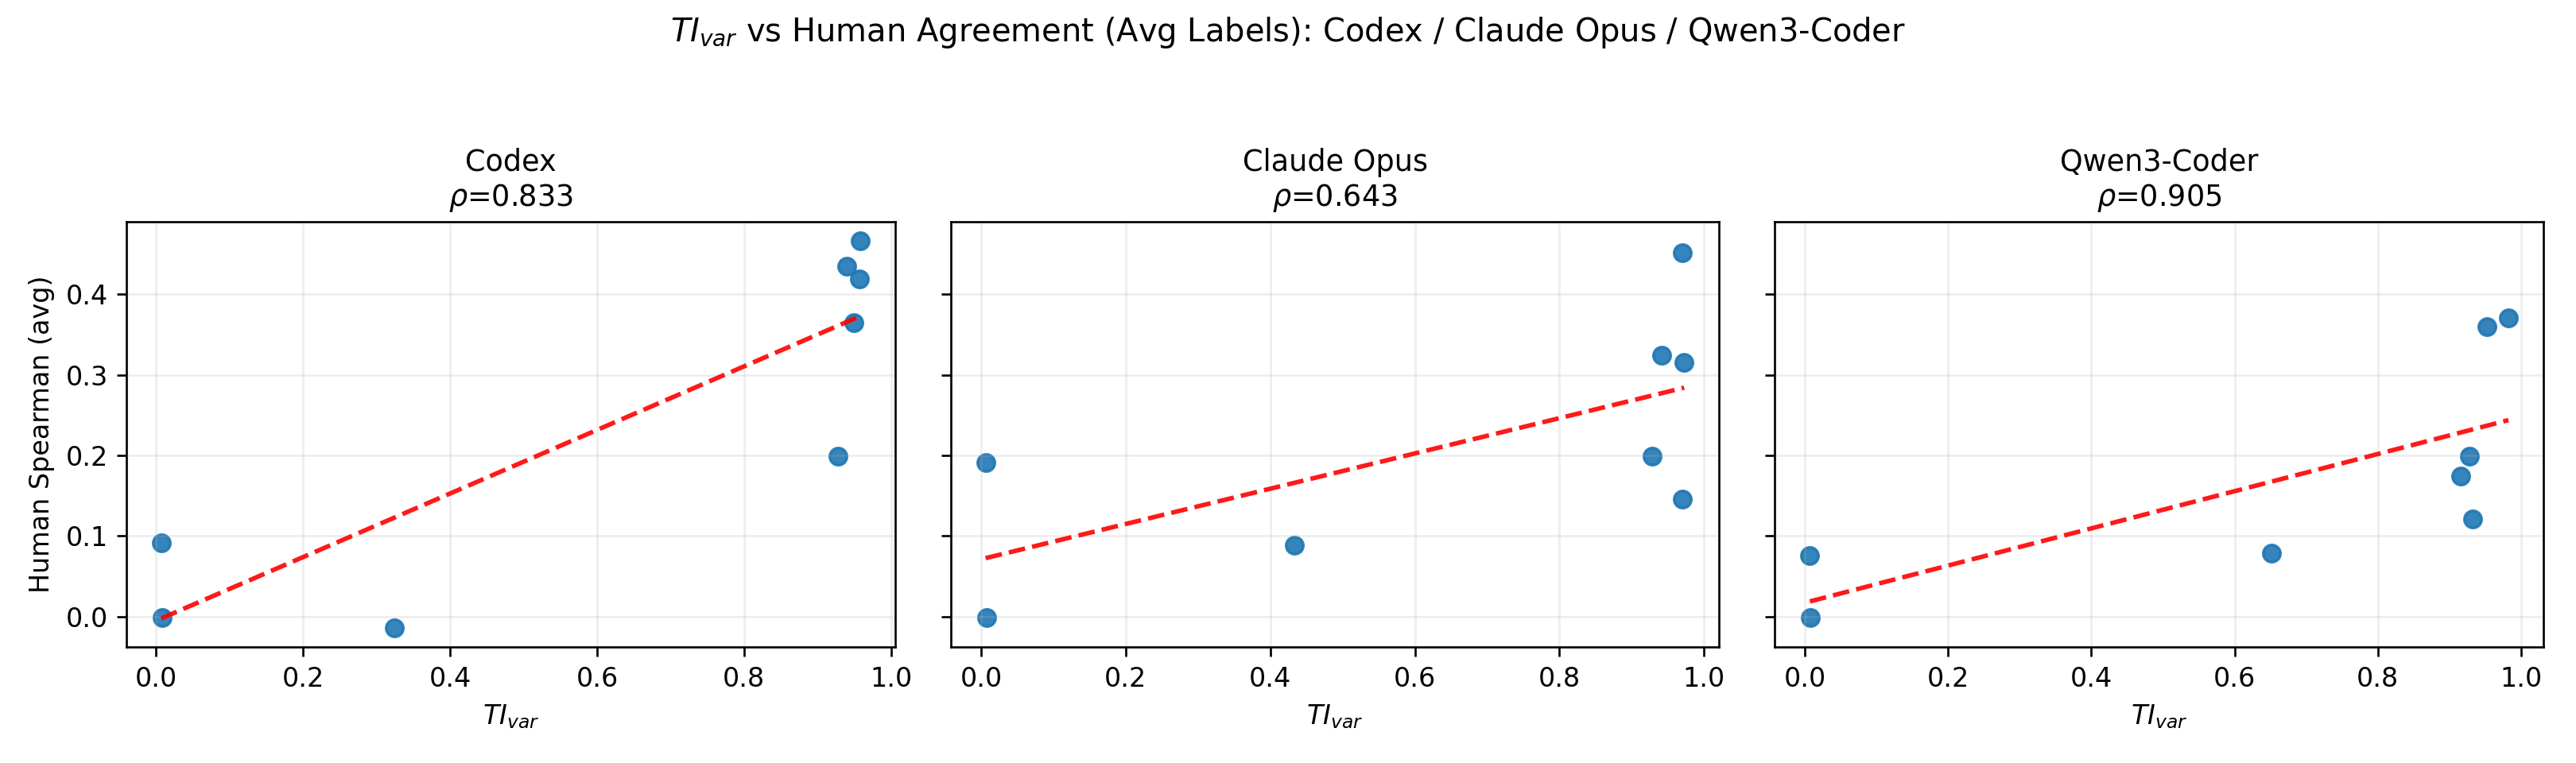
\includegraphics[width=\linewidth]{figures/fig_tivar_scatter_3models_avg.png}
      \caption{Each point is one judge configuration: higher \tivar{} $\rightarrow$ higher human agreement, in \textbf{all three judge families} (avg labels).}
    \end{figure}

    \textbf{Catches what agreement alone misses:} an intentionally broken judge (\textsc{Bad-Stringy}) still reaches ${\approx}0.45$ human Spearman, yet fails weak monotonicity ($12.5\%$) --- \tivar{} flags it.

  \end{block}

  % CS197 move 5 (evidence the properties are real + honest failure mode)
  \begin{block}{Stress tests keep the judge honest}

    \begin{figure}
      \centering
      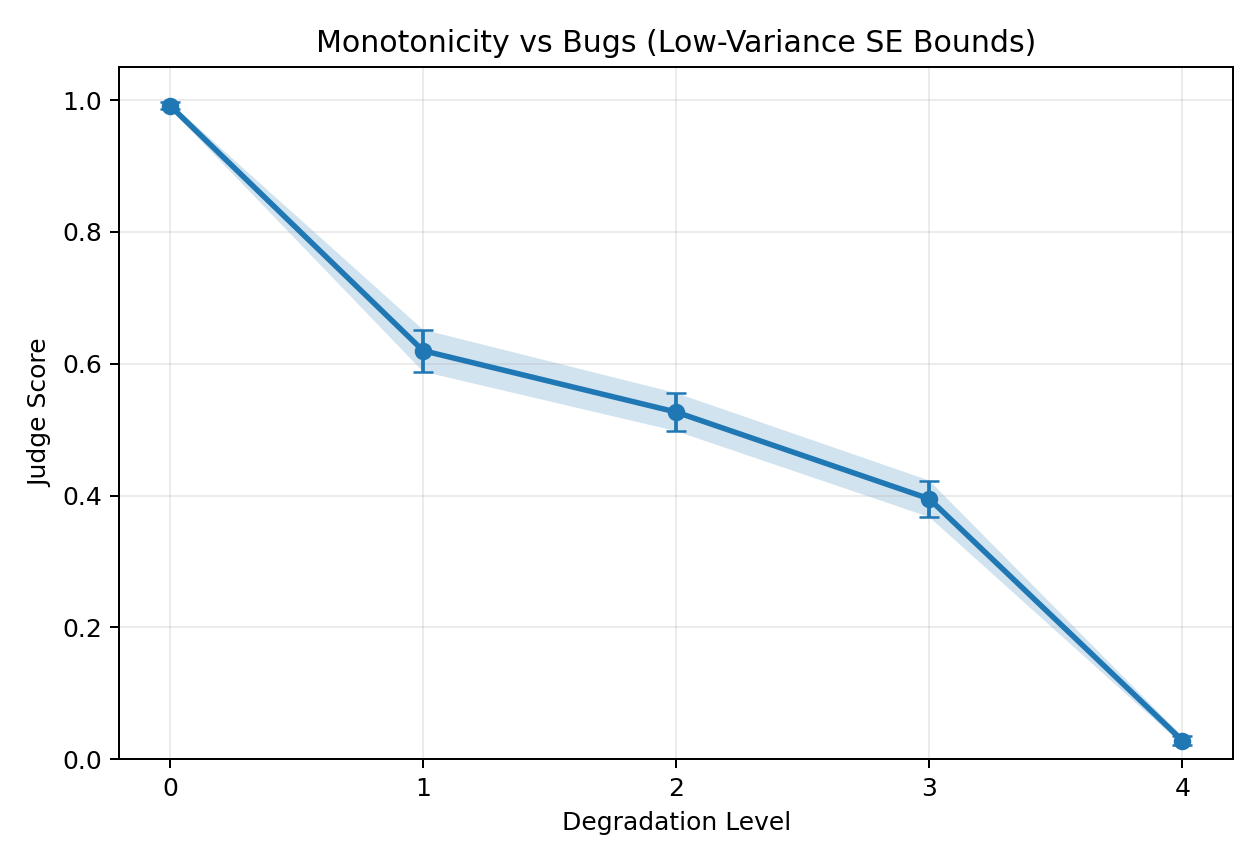
\includegraphics[width=0.49\linewidth]{figures/monotonicity_bugs_lowvar_se_bounds.png}\hfill
      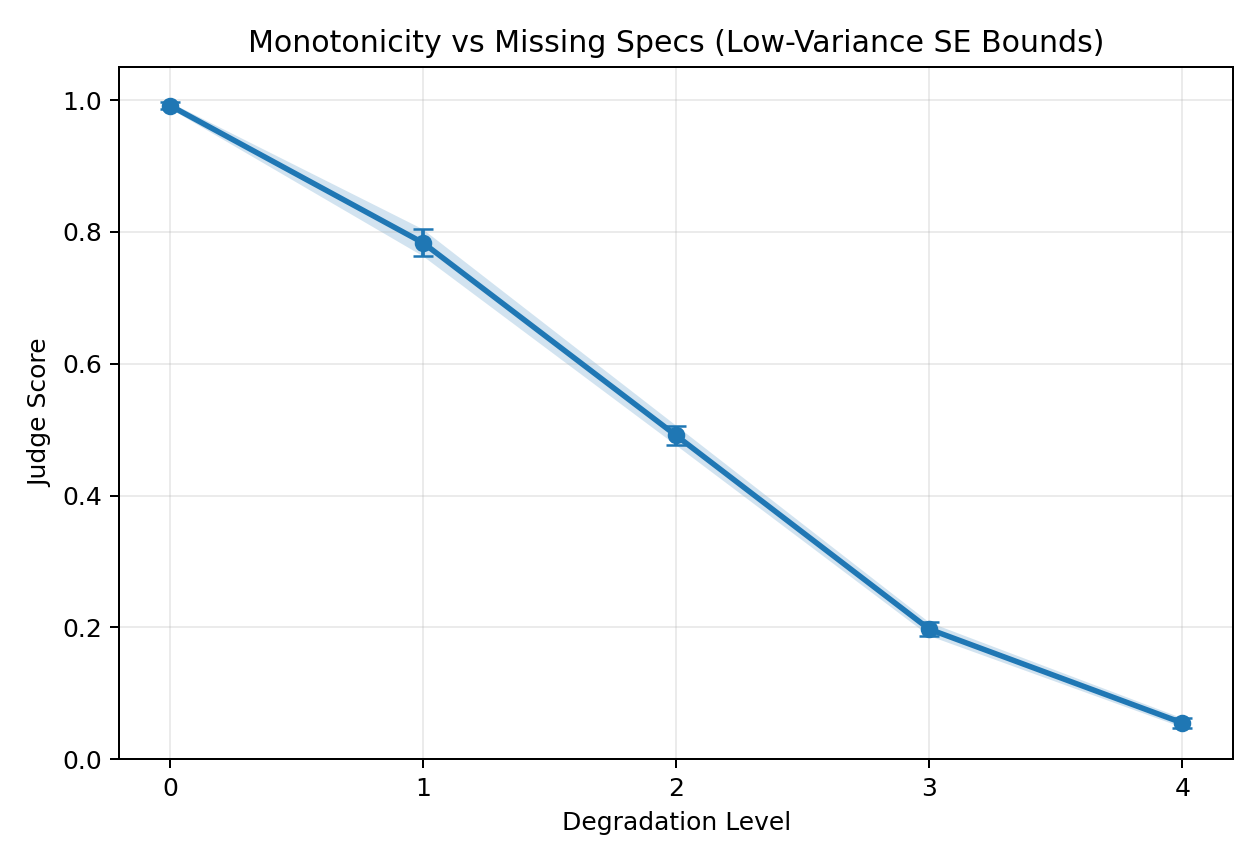
\includegraphics[width=0.49\linewidth]{figures/monotonicity_missing_specs_lowvar_se_bounds.png}
      \caption{GPT-5.3-Codex judge, 184 \textsc{VeriBench} files: scores fall as bugs are injected (left, $\rho=-0.808$) and as specs are deleted (right, $\rho=-0.899$).}
    \end{figure}

    \textbf{Known failure mode:} aggressive $\alpha$-renaming scores $0.399$ vs.\ $\geq 0.849$ for milder semantics-preserving rewrites --- LLM judges key on surface strings the Lean kernel ignores.

  \end{block}

  % CS197 move 5 (downstream use)
  \begin{block}{The certified judge ranks theorem-generation agents}

    On \textsc{VeriBench}, the calibrated judge ranks feedback-driven agents above plain prompting (avg normalized score): \textbf{DSPy ReAct 0.615} $>$ Trace++ 0.588 $>$ Trace+ 0.477 $>$ \textbf{baseline 0.470} --- a downstream sanity check, not independent proof of correctness.

  \end{block}

  % CS197 move 6: takeaways — vision, not self-congratulation; caveat is part of the claim
  \begin{alertblock}{Takeaways}

    \begin{itemize}
      \item \textbf{Amortized oversight:} one $n{=}75$ human panel + automated falsifiable checks screen every new judge configuration --- no re-labeling.
      \item \textbf{Measure trust, don't assume it:} behavioral properties expose failures (broken baselines, $\alpha$-renaming brittleness) that human-agreement scores miss.
      \item \textbf{Scope:} \emph{validation-set calibration evidence, not universal reliability} --- a locked held-out test on an independent pool (5 raters, 343 labels, 78 pairs) is next.
    \end{itemize}

  \end{alertblock}

  \begin{block}{References}

    \nocite{*}
    \begin{minipage}[c]{0.74\linewidth}
      \footnotesize{\bibliographystyle{plain}\bibliography{poster}}
    \end{minipage}\hfill
    \begin{minipage}[c]{0.22\linewidth}
      \centering
      \qrcode[height=4cm]{https://github.com/brando90/cert-judge}\\[0.8ex]
      {\small \textbf{Code}}
      % TODO: arXiv link when live
    \end{minipage}

  \end{block}

\end{column}

\separatorcolumn
\end{columns}
\end{frame}

\end{document}
